\documentclass[tikz]{standalone}
\usetikzlibrary{calc}
\begin{document}
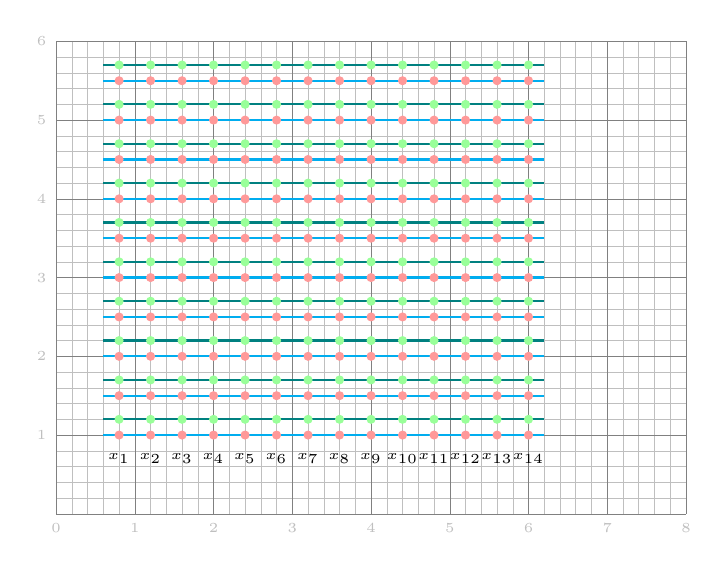
\begin{tikzpicture}
  % Help lines
  \draw[help lines,step=.2,gray!50] (0,0) grid (8,6);
  \draw[help lines] (0,0) grid (8,6);
  \foreach \x in {0, 1, ..., 8} \node[below, gray!50] at (\x,0){\tiny{\x}};
  \foreach \y in {1, 2, ..., 6} \node[left, gray!50] at (0,\y){\tiny{\y}};
  \foreach \y in {1, 2, ..., 5}{
    \draw[thick, cyan](0.6, \y)--(6.2, \y);
    \draw[thick, teal](0.6, \y+0.2)--(6.2, \y+0.2);
    \draw[thick, cyan](0.6, \y+0.5)--(6.2, \y+0.5);
    \draw[thick, teal](0.6, \y+0.7)--(6.2, \y+0.7);
    \foreach \x in {0.8, 1.2, ..., 6}{
      \draw[fill, red!40!white] (\x, \y) circle (0.05);
      \draw[fill, green!40!white] (\x, \y+.2) circle (0.05);
      \draw[fill, red!40!white] (\x, \y+.5) circle (0.05);
      \draw[fill, green!40!white] (\x, \y+.7) circle (.05);
    }
  }
  \foreach \x in {1, 2, ..., 14} \node at (0.4+\x*.4, 0.7) {\tiny $x_{\x}$};
\end{tikzpicture}
\end{document}
